\documentclass{beamer}
\usepackage{amsmath,graphics}
\usepackage{amssymb}

\usetheme{default}
\usepackage{xcolor}

\definecolor{solarizedBase03}{HTML}{002B36}
\definecolor{solarizedBase02}{HTML}{073642}
\definecolor{solarizedBase01}{HTML}{586e75}
\definecolor{solarizedBase00}{HTML}{657b83}
\definecolor{solarizedBase0}{HTML}{839496}
\definecolor{solarizedBase1}{HTML}{93a1a1}
\definecolor{solarizedBase2}{HTML}{EEE8D5}
\definecolor{solarizedBase3}{HTML}{FDF6E3}
\definecolor{solarizedYellow}{HTML}{B58900}
\definecolor{solarizedOrange}{HTML}{CB4B16}
\definecolor{solarizedRed}{HTML}{DC322F}
\definecolor{solarizedMagenta}{HTML}{D33682}
\definecolor{solarizedViolet}{HTML}{6C71C4}
%\definecolor{solarizedBlue}{HTML}{268BD2}
\definecolor{solarizedBlue}{HTML}{134676}
\definecolor{solarizedCyan}{HTML}{2AA198}
\definecolor{solarizedGreen}{HTML}{859900}
\definecolor{myBlue}{HTML}{162DB0}%{261CA4}
\setbeamercolor*{item}{fg=myBlue}
\setbeamercolor{normal text}{fg=solarizedBase03, bg=solarizedBase3}
\setbeamercolor{alerted text}{fg=myBlue}
\setbeamercolor{example text}{fg=myBlue, bg=solarizedBase3}
\setbeamercolor*{frametitle}{fg=solarizedRed}
\setbeamercolor*{title}{fg=solarizedRed}
\setbeamercolor{block title}{fg=myBlue, bg=solarizedBase3}
\setbeameroption{hide notes}
\setbeamertemplate{note page}[plain]
\beamertemplatenavigationsymbolsempty
\usefonttheme{professionalfonts}
\usefonttheme{serif}

\usepackage{fourier}

\def\vec#1{\mathchoice{\mbox{\boldmath$\displaystyle#1$}}
{\mbox{\boldmath$\textstyle#1$}}
{\mbox{\boldmath$\scriptstyle#1$}}
{\mbox{\boldmath$\scriptscriptstyle#1$}}}
\definecolor{OwnGrey}{rgb}{0.560,0.000,0.000} % #999999
\definecolor{OwnBlue}{rgb}{0.121,0.398,0.711} % #1f64b0
\definecolor{red4}{rgb}{0.5,0,0}
\definecolor{blue4}{rgb}{0,0,0.5}
\definecolor{Blue}{rgb}{0,0,0.66}
\definecolor{LightBlue}{rgb}{0.9,0.9,1}
\definecolor{Green}{rgb}{0,0.5,0}
\definecolor{LightGreen}{rgb}{0.9,1,0.9}
\definecolor{Red}{rgb}{0.9,0,0}
\definecolor{LightRed}{rgb}{1,0.9,0.9}
\definecolor{White}{gray}{1}
\definecolor{Black}{gray}{0}
\definecolor{LightGray}{gray}{0.8}
\definecolor{Orange}{rgb}{0.1,0.2,1}
\setbeamerfont{sidebar right}{size=\scriptsize}
\setbeamercolor{sidebar right}{fg=Black}

\renewcommand{\emph}[1]{{\textcolor{solarizedRed}{\itshape #1}}}

\newcommand\cA{\mathcal A}
\newcommand\cB{\mathcal B}
\newcommand\cC{\mathcal C}
\newcommand\cD{\mathcal D}
\newcommand\cE{\mathcal E}
\newcommand\cF{\mathcal F}
\newcommand\cG{\mathcal G}
\newcommand\cH{\mathcal H}
\newcommand\cI{\mathcal I}
\newcommand\cJ{\mathcal J}
\newcommand\cK{\mathcal K}
\newcommand\cL{\mathcal L}
\newcommand\cM{\mathcal M}
\newcommand\cN{\mathcal N}
\newcommand\cO{\mathcal O}
\newcommand\cP{\mathcal P}
\newcommand\cQ{\mathcal Q}
\newcommand\cR{\mathcal R}
\newcommand\cS{\mathcal S}
\newcommand\cT{\mathcal T}
\newcommand\cU{\mathcal U}
\newcommand\cV{\mathcal V}
\newcommand\cW{\mathcal W}
\newcommand\cX{\mathcal X}
\newcommand\cY{\mathcal Y}
\newcommand\cZ{\mathcal Z}

\newcommand\fA{\mathfrak A}
\newcommand\fB{\mathfrak B}
\newcommand\fC{\mathfrak C}
\newcommand\fD{\mathfrak D}
\newcommand\fE{\mathfrak E}
\newcommand\fF{\mathfrak F}
\newcommand\fG{\mathfrak G}
\newcommand\fH{\mathfrak H}
\newcommand\fI{\mathfrak I}
\newcommand\fJ{\mathfrak J}
\newcommand\fK{\mathfrak K}
\newcommand\fL{\mathfrak L}
\newcommand\fM{\mathfrak M}
\newcommand\fN{\mathfrak N}
\newcommand\fO{\mathfrak O}
\newcommand\fP{\mathfrak P}
\newcommand\fQ{\mathfrak Q}
\newcommand\fR{\mathfrak R}
\newcommand\fS{\mathfrak S}
\newcommand\fT{\mathfrak T}
\newcommand\fU{\mathfrak U}
\newcommand\fV{\mathfrak V}
\newcommand\fW{\mathfrak W}
\newcommand\fX{\mathfrak X}
\newcommand\fY{\mathfrak Y}
\newcommand\fZ{\mathfrak Z}

\newcommand\fa{\mathfrak a}
\newcommand\fb{\mathfrak b}
\newcommand\fc{\mathfrak c}
\newcommand\fd{\mathfrak d}
\newcommand\fe{\mathfrak e}
\newcommand\ff{\mathfrak f}
\newcommand\fg{\mathfrak g}
\newcommand\fh{\mathfrak h}
%\newcommand\fi{\mathfrak i}
\newcommand\fj{\mathfrak j}
\newcommand\fk{\mathfrak k}
\newcommand\fl{\mathfrak l}
\newcommand\fm{\mathfrak m}
\newcommand\fn{\mathfrak n}
\newcommand\fo{\mathfrak o}
\newcommand\fp{\mathfrak p}
\newcommand\fq{\mathfrak q}
\newcommand\fr{\mathfrak r}
\newcommand\fs{\mathfrak s}
\newcommand\ft{\mathfrak t}
\newcommand\fu{\mathfrak u}
\newcommand\fv{\mathfrak v}
\newcommand\fw{\mathfrak w}
\newcommand\fx{\mathfrak x}
\newcommand\fy{\mathfrak y}
\newcommand\fz{\mathfrak z}

\newcommand\vA{\vec A}
\newcommand\vB{\vec B}
\newcommand\vC{\vec C}
\newcommand\vD{\vec D}
\newcommand\vE{\vec E}
\newcommand\vF{\vec F}
\newcommand\vG{\vec G}
\newcommand\vH{\vec H}
\newcommand\vI{\vec I}
\newcommand\vJ{\vec J}
\newcommand\vK{\vec K}
\newcommand\vL{\vec L}
\newcommand\vM{\vec M}
\newcommand\vN{\vec N}
\newcommand\vO{\vec O}
\newcommand\vP{\vec P}
\newcommand\vQ{\vec Q}
\newcommand\vR{\vec R}
\newcommand\vS{\vec S}
\newcommand\vT{\vec T}
\newcommand\vU{\vec U}
\newcommand\vV{\vec V}
\newcommand\vW{\vec W}
\newcommand\vX{\vec X}
\newcommand\vY{\vec Y}
\newcommand\vZ{\vec Z}

\newcommand\va{\vec a}
\newcommand\vb{\vec b}
\newcommand\vc{\vec c}
\newcommand\vd{\vec d}
\newcommand\ve{\vec e}
\newcommand\vf{\vec f}
\newcommand\vg{\vec g}
\newcommand\vh{\vec h}
\newcommand\vi{\vec i}
\newcommand\vj{\vec j}
\newcommand\vk{\vec k}
\newcommand\vl{\vec l}
\newcommand\vm{\vec m}
\newcommand\vn{\vec n}
\newcommand\vo{\vec o}
\newcommand\vp{\vec p}
\newcommand\vq{\vec q}
\newcommand\vr{\vec r}
\newcommand\vs{\vec s}
\newcommand\vt{\vec t}
\newcommand\vu{\vec u}
\newcommand\vv{\vec v}
\newcommand\vw{\vec w}
\newcommand\vx{\vec x}
\newcommand\vy{\vec y}
\newcommand\vz{\vec z}

\renewcommand\AA{\mathbb A}
\newcommand\NN{\mathbb N}
\newcommand\ZZ{\mathbb Z}
\newcommand\PP{\mathbb P}
\newcommand\QQ{\mathbb Q}
\newcommand\RR{\mathbb R}
\renewcommand\SS{\mathbb S}
\newcommand\CC{\mathbb C}

\newcommand{\ord}{\mathrm{ord}}
\newcommand{\id}{\mathrm{id}}
\newcommand{\pr}{\mathrm{P}}
\newcommand{\Vol}{\mathrm{vol}}
\newcommand\norm[1]{\left\|{#1}\right\|} 
\newcommand\sign{\mathrm{sign}}
\newcommand{\eps}{\varepsilon}
\newcommand{\abs}[1]{\left|#1\right|}
\newcommand\bc[1]{\left({#1}\right)} 
\newcommand\cbc[1]{\left\{{#1}\right\}} 
\newcommand\bcfr[2]{\bc{\frac{#1}{#2}}} 
\newcommand{\bck}[1]{\left\langle{#1}\right\rangle} 
\newcommand\brk[1]{\left\lbrack{#1}\right\rbrack} 
\newcommand\scal[2]{\bck{{#1},{#2}}} 
\newcommand{\vecone}{\mathbb{1}}
\newcommand{\tensor}{\otimes}
\newcommand{\diag}{\mathrm{diag}}
\newcommand{\ggt}{\mathrm{ggT}}
\newcommand{\kgv}{\mathrm{kgV}}
\newcommand{\trans}{\top}

\newcommand{\Karonski}{Karo\'nski}
\newcommand{\Erdos}{Erd\H{o}s}
\newcommand{\Renyi}{R\'enyi}
\newcommand{\Lovasz}{Lov\'asz}
\newcommand{\Juhasz}{Juh\'asz}
\newcommand{\Bollobas}{Bollob\'as}
\newcommand{\Furedi}{F\"uredi}
\newcommand{\Komlos}{Koml\'os}
\newcommand{\Luczak}{\L uczak}
\newcommand{\Kucera}{Ku\v{c}era}
\newcommand{\Szemeredi}{Szemer\'edi}

\renewcommand{\ae}{\"a}
\renewcommand{\oe}{\"o}
\newcommand{\ue}{\"u}
\newcommand{\Ae}{\"A}
\newcommand{\Oe}{\"O}
\newcommand{\Ue}{\"U}

\newcommand{\im}{\mathrm{im}}
\newcommand{\rrk}{\mathrm{zrg}}
\newcommand{\crk}{\mathrm{srg}}
\newcommand{\rk}{\mathrm{rg}}
\newcommand{\GL}{\mathrm{GL}}
\newcommand{\SL}{\mathrm{SL}}
\newcommand{\SO}{\mathrm{SO}}

\newcommand{\mytitle}{Orthogonalit\ae t}

\title[Linadi]{\mytitle}
\author[Amin Coja-Oghlan]{Amin Coja-Oghlan}
\institute[Frankfurt]{JWGUFFM}
\date{}

\begin{document}

\frame[plain]{\titlepage}

\begin{frame}\frametitle{\mytitle}
	\begin{block}{Definition}
		\begin{itemize}
			\item Zwei Vektoren $v,w\in\RR^n$ sind \emph{orthogonal} (Schreibweise: $v\perp w$), falls
				\begin{align*}
				v^\trans w=0.
				\end{align*}
			\item Vektoren $v_1,\ldots,v_\ell$ hei\ss en \emph{orthogonal}, falls
				\begin{align*}
					v_i\perp v_j&&\mbox{f\ue r alle }1\leq i<j\leq n.
				\end{align*}
			\item Ein Vektor $v\in\RR^n$ ist ein \emph{Einheitsvektor}, falls
				\begin{align*}
				v^\trans v=1.
				\end{align*}
				{\itshape Das ist \ae quivalent zu $\|v\|=1$.}
		\end{itemize}
	\end{block}
\end{frame}

\begin{frame}\frametitle{\mytitle}
	\begin{block}{Definition}
		\begin{itemize}
			\item Ein Vektor $v\in\RR^n$ ist ein \emph{Einheitsvektor}, falls
				\begin{align*}
				v^\trans v=1.
				\end{align*}
				{\itshape Das ist \ae quivalent zu $\|v\|=1$.}
			\item Vektoren $v_1,\ldots,v_\ell$ hei\ss en \emph{orthonormal}, falls $v_1,\ldots,v_\ell$ orthogonale Einheitsvektoren sind.
		\end{itemize}
	\end{block}
\end{frame}

\begin{frame}\frametitle{\mytitle}
	\begin{block}{Definition}
		Sei $E\subseteq\RR^n$ ein Untervektorraum.
Vektoren $v_1,\ldots,v_\ell$ nennen wir eine \emph{Orthonormalbasis} von $E$, falls
		\begin{itemize}
			\item $v_1,\ldots,v_\ell$ orthonormal sind und
			\item $v_1,\ldots,v_\ell$ eine Basis von $E$ ist.
		\end{itemize}
	\end{block}
\end{frame}

\begin{frame}\frametitle{\mytitle}
	\hfill\includegraphics[height=30mm]{pics/basis.pdf}
	\begin{block}{Beispiel}
		\begin{itemize}
			\item Die Vektoren $\binom 10$, $\binom 01$ sind eine Orthonormalbasis von $\RR^2$.
			\item Die Vektoren $\binom{\sqrt 2/2}{\sqrt 2/2},\binom{-\sqrt 2/2}{\sqrt 2/2}$ sind ebenfalls eine Orthonormalbasis von $\RR^2$.
			\item Die Vektoren $\binom 20$, $\binom 0{1/2}$ eine orthogonal aber nicht orthonormal.
		\end{itemize}
	\end{block}
\end{frame}

\begin{frame}\frametitle{\mytitle}
	\begin{block}{Beispiel}
		\begin{itemize}
			\item Die Vektoren
				\begin{align*}
				\begin{pmatrix}1\\0\\0 \end{pmatrix},
				\begin{pmatrix}0\\-1\\0 \end{pmatrix}\in\RR^3
				\end{align*}
				sind orthonormal aber keine Orthonormalbasis von $\RR^3$.
			\item Sie bilden aber eine Orthonormalbasis des Untervektorraums
				\begin{align*}
					E&=\cbc{\begin{pmatrix}x\\y\\0\end{pmatrix}:x,y\in\RR}
				\end{align*}
		\end{itemize}
	\end{block}
\end{frame}

\begin{frame}\frametitle{\mytitle}
	\begin{block}{Proposition}
		Wenn die Vektoren $v_1,\ldots,v_\ell$ orthonormal sind, dann sind sie linear unabh\ae ngig.
	\end{block}
\end{frame}

\begin{frame}\frametitle{\mytitle}
	\begin{block}{Satz}
		Sei $E\subseteq\RR^n$ ein Untervektorraum mit $k=\dim(E)$ und seien $v_1,\ldots,v_\ell\in E$ orthonormal.
		Dann gibt es Vektoren $v_{\ell+1},\ldots,v_k$, so da\ss\ $v_1,\ldots,v_k$ eine Orthonormalbasis von $E$ ist.
	\end{block}
	\begin{block}{Korollar}
		Jeder Untervektorraum $E\subseteq\RR^n$ besitzt eine Orthonormalbasis.
	\end{block}
\end{frame}

\begin{frame}\frametitle{\mytitle}
	\begin{block}{Gram-Schmidt-Orthogonalisierungsschema}
	\begin{itemize}
	\item Seien $u_1,\ldots,u_\ell$ linear unabh\ae ngige Vektoren.
	\item \emph{Ziel:} Konstruktion einer Orthonormalbasis $v_1,\ldots,v_\ell$ von $\bck{u_1,\ldots,u_\ell}$. 
	\item Zun\ae chst definiere $v_1=\|u_1\|^{-1}u_1$; dann gilt $\|v_1\|=1$.
	\item F\ue r $i=2,\ldots,\ell$ gehe wie folgt vor:
	\item $\quad$Bestimme $v_i'=u_i-\sum_{j=1}^{i-1}u_i^\trans v_i\cdot v_i$.
	\item $\quad$Definiere $v_i=v_i'/\|v_i'\|$.
	\end{itemize}
	\end{block}
\end{frame}

\begin{frame}\frametitle{\mytitle}
	\begin{block}{Beispiel}
	\begin{itemize}
		\item Lineare unabh\ae ngige Vektoren:
\begin{align*}
	u_1&=\begin{pmatrix}1\\1\\0\end{pmatrix}&
	u_2&=\begin{pmatrix}1\\1\\-4\end{pmatrix}&
	u_3&=\begin{pmatrix} 2\\-1\\1 \end{pmatrix}
\end{align*}
\item Wir berechnen $\|u_1\|=\sqrt{u_1^\trans u_1}=\sqrt{1\cdot 1+1\cdot 1+0\cdot0}=\sqrt 2$.
\item Also 
	\begin{align*}
		v_1&=2^{-1/2}u_1=\begin{pmatrix}1/\sqrt 2\\1/\sqrt 2\\0\end{pmatrix}
	\end{align*}
\end{itemize}
	\end{block}
\end{frame}

\begin{frame}\frametitle{\mytitle}
	\begin{block}{Beispiel}
	\begin{itemize}
\item Als n\ae chstes berechnen wir 
	\begin{align*}
		v_2'&=u_2-u_2^\trans v_1\cdot v_1=\begin{pmatrix}1\\1\\-4\end{pmatrix}-\begin{pmatrix}1&1&-4\end{pmatrix}\cdot\begin{pmatrix}1/\sqrt 2\\1/\sqrt 2\\0\end{pmatrix}\cdot\begin{pmatrix}1/\sqrt 2\\1/\sqrt 2\\0\end{pmatrix}\\
			&=\begin{pmatrix}1\\1\\-4\end{pmatrix}-\bc{1\cdot 2^{-1/2}+1\cdot 2^{-1/2}+(-4)\cdot 0}\begin{pmatrix}1/\sqrt 2\\1/\sqrt 2\\0\end{pmatrix}\\
			&=\begin{pmatrix}1\\1\\-4\end{pmatrix}-\sqrt 2\begin{pmatrix}1/\sqrt 2\\1/\sqrt 2\\0\end{pmatrix}
			=\begin{pmatrix}1\\1\\-4\end{pmatrix}-\begin{pmatrix}1\\1\\0\end{pmatrix}=\begin{pmatrix}0\\0\\-4\end{pmatrix}
	\end{align*}
	\item Weil $\|v_2'\|=4$, erhalten wir $ v_2=\frac{1}{4}v_2'=\begin{pmatrix}0\\0\\-1\end{pmatrix} $.
\end{itemize}
	\end{block}
\end{frame}

\begin{frame}\frametitle{\mytitle}
	\begin{block}{Beispiel}
		\begin{itemize}
			\item Ferner berechnen wir
				\begin{align*}
					v_3'&=u_3-u_3v_1\cdot v_1-u_3v_2\cdot v_2\\
						&=\begin{pmatrix} 2\\-1\\1 \end{pmatrix}-
					\begin{pmatrix} 2&-1&1 \end{pmatrix}\begin{pmatrix}1/\sqrt 2\\1/\sqrt 2\\0\end{pmatrix}\cdot\begin{pmatrix}1/\sqrt 2\\1/\sqrt 2\\0\end{pmatrix}-\begin{pmatrix} 2&-1&1 \end{pmatrix}\begin{pmatrix}0\\0\\-1\end{pmatrix}\begin{pmatrix}0\\0\\-1\end{pmatrix}\\
									 &=\begin{pmatrix} 2\\-1\\1 \end{pmatrix}-\bc{\frac{2}{\sqrt 2}-\frac{1}{\sqrt 2}}\begin{pmatrix}1/\sqrt 2\\1/\sqrt 2\\0\end{pmatrix}+1\cdot\begin{pmatrix}0\\0\\-1\end{pmatrix}\\
									 &=\begin{pmatrix} 2\\-1\\1 \end{pmatrix}-\begin{pmatrix}1/2\\1/2\\0\end{pmatrix}+\begin{pmatrix}0\\0\\-1\end{pmatrix}=\begin{pmatrix}3/2\\-3/2\\0\end{pmatrix}
				\end{align*}
		\end{itemize}
	\end{block}
\end{frame}

\begin{frame}\frametitle{\mytitle}
	\begin{block}{Beispiel}
		\begin{itemize}
			\item Schlie\ss lich erhalten wir
				\begin{align*}
					v_3&=\|v_3'\|^{-1}v_3'=\frac{1}{\sqrt{(3/2)^2+(-3/2)^2+0^2}}\begin{pmatrix}3/2\\-3/2\\0\end{pmatrix}=\begin{pmatrix}1/\sqrt 2\\-1/\sqrt 2\\0\end{pmatrix}
				\end{align*}
			\item Das Ergebnis sind also die drei orthonormalen Vektoren
				\begin{align*}
					\begin{pmatrix}1/\sqrt 2\\1/\sqrt 2\\0\end{pmatrix},\quad\begin{pmatrix}0\\0\\-1\end{pmatrix},\quad\begin{pmatrix}1/\sqrt 2\\-1/\sqrt 2\\0\end{pmatrix}
				\end{align*}
		\end{itemize}
	\end{block}
\end{frame}

\begin{frame}\frametitle{\mytitle}
	\begin{block}{Definition}
		Eine $n\times n$-Matrix $A$ hei\ss t \emph{orthogonal}, falls $A^\trans A=\id_n.$
	\end{block}
\end{frame}

\begin{frame}\frametitle{\mytitle}
	\begin{block}{Proposition}
		Sei $A$ eine $n\times n$-Matrix.
		Die folgenden Aussagen sind \ae quivalent.
		\begin{itemize}
			\item $A$ ist orthogonal.
			\item $A$ ist invertierbar und $A^{-1}=A^\trans$.
			\item Die Spalten von $A$ sind eine Orthonormalbasis von $\RR^n$.
			\item F\ue r alle Vektoren $u,v\in\RR^n$ gilt $(Au)^\trans(Av)=u^\trans v$.
			\item F\ue r alle Vektoren $u\in\RR^n$ gilt $\|Au\|=\|u\|$.
		\end{itemize}
	\end{block}
\end{frame}

\begin{frame}\frametitle{\mytitle}
	\begin{block}{Beispiel}
	\begin{itemize}
	\item Die Matrix $\id_2=\begin{pmatrix}1&0\\0&1\end{pmatrix}$ ist orthogonal.
	\item Allgemeiner ist f\ue r jedes $n\in\NN$ die Einheitsmatrix $\id_n$ orthogonal.
	\item Die Matrizen $ \begin{pmatrix}1&0\\0&-1\end{pmatrix},\ \begin{pmatrix}0&1\\-1&0\end{pmatrix} $
		sind orthogonal.
	\item Die Matrix
		\begin{align*}
		\begin{pmatrix}
			1/\sqrt 2&0&1/\sqrt 2\\1/\sqrt 2&0&-1/\sqrt 2\\0&-1&0
		\end{pmatrix}
		\end{align*}
		ist orthogonal.
	\end{itemize}
	\end{block}
\end{frame}

\begin{frame}\frametitle{\mytitle}
	\begin{block}{Proposition}
		Die Menge $O(n)$ der orthogonalen $n\times n$-Matrizen bildet eine Untergruppe von $\GL(n)$.
	\end{block}
	\begin{block}{Proposition}
		Die Menge $\SL(n)$ der Matrizen $A\in\GL(n)$ mit $\det(A)=1$ ist eine Untergruppe von $\GL(n)$.
	\end{block}
	\begin{block}{Proposition}
		Die Menge $\SO(n)=O(n)\cap\SL(n)$ der orthogonalen Matrizen $A$ mit $\det(A)=1$ ist eine Untergruppe von $\GL(n)$.
	\end{block}
	{\itshape Wir nennen $\SL(n)$ die spezielle lineare Gruppe und $\SO(n)$ die spezielle orthogonale Gruppe.}
\end{frame}

\begin{frame}\frametitle{\mytitle}
	\begin{block}{Beispiel}
		\begin{itemize}
			\item Die Matrix 
				\begin{align*}
					\begin{pmatrix} \cos(\alpha)&-\sin(\alpha)\\\sin(\alpha)&\cos(\alpha) \end{pmatrix}\in\SO(2)
				\end{align*}
				stellt die Rotation um den Winkel $\alpha$ dar.
			\item Die Matrizen
				\begin{align*}
					\begin{pmatrix} -1&0\\0&1 \end{pmatrix},\qquad
					\begin{pmatrix} 1&0\\0&-1 \end{pmatrix}\in O(2)
				\end{align*}
				stellen Spiegelungen dar.
			\item Weil $O(n)$ eine Gruppe sind, sind beliebige Produkte dieser Matrizen orthogonal.
		\end{itemize}
	\end{block}
\end{frame}

\begin{frame}\frametitle{\mytitle}
	\begin{block}{Basiswechsel}
		\begin{itemize}
			\item Sei $A$ eine orthogonale $n\times n$-Matrix.
			\item Seien $v_1,\ldots,v_n$ die Spaltenvektoren von $A$.
			\item Sei ferner $u\in\RR^n$.
			\item Dann ist
				\begin{align*}
					Au&=\sum_{i=1}^nu_iv_i.
				\end{align*}
			\item Wir k\oe nnen uns also $Au$ also den Vektor mit den Koordinaten $u$ in dem Koordinatensystem $v_1,\ldots,v_n$ vorstellen.
		\end{itemize}
	\end{block}
\end{frame}

\begin{frame}\frametitle{\mytitle}
	\begin{block}{Basiswechsel}
		\begin{itemize}
			\item Umgekehrt k\oe nnen wir f\ue r einen gegebenen Vektor $y\in\RR^n$ immer einen Vektor $u\in\RR^n$ finden, so da\ss\ $y=Au$, n\ae mlich
				\begin{align*}
					u=A^{-1}y.
				\end{align*}
			\item Weil $A$ orthogonal ist, gilt $A^{-1}=A^\trans$ und wir k\oe nnen $u$ leicht ausrechnen:
				\begin{align*}
					u&=A^\trans y&\Rightarrow&&u_i=&y^\trans v_i.
				\end{align*}
			\item Die Zaheln $u_i=y^\trans v_i$ werden die \emph{Fourierkoeffizienten} von $y$ bzgl.\ der Orthonormalbasis $v_1,\ldots,v_n$ genannt.
			\item Geometrisch ist $y^\trans v_i$ die Projektion von $y$ auf die durch $v_i$ definierte Gerade.
		\end{itemize}
	\end{block}
\end{frame}

\begin{frame}\frametitle{\mytitle}
	\begin{block}{Beispiel}
		\begin{itemize}
			\item Wir betrachten die Orthonormalbasis
\begin{align*}
					\begin{pmatrix}1/\sqrt 2\\1/\sqrt 2\\0\end{pmatrix},\quad\begin{pmatrix}0\\0\\-1\end{pmatrix},\quad\begin{pmatrix}1/\sqrt 2\\-1/\sqrt 2\\0\end{pmatrix}
				\end{align*}
			\item Die entsprechende orthogonale Matrix lautet
				\begin{align*}
				A=\begin{pmatrix} 1/\sqrt 2&0&1/\sqrt 2\\1/\sqrt 2&0&-1/\sqrt 2\\0&-1&0 \end{pmatrix}
				\end{align*}
			\item Die inverse Matrix lautet
				\begin{align*}
					A^\trans=\begin{pmatrix} 1/\sqrt 2&1/\sqrt 2&0\\0&0&-1\\1/\sqrt 2&-1/\sqrt 2&0 \end{pmatrix}
				\end{align*}
		\end{itemize}
	\end{block}
\end{frame}

\begin{frame}\frametitle{\mytitle}
	\begin{block}{Beispiel}
		\begin{itemize}
			\item Betrachte nun den Vektor $y=\begin{pmatrix}1\\2\\3\end{pmatrix}$
			\item Wir bestimmen 
				\begin{align*}
					u&=A^\trans y=\begin{pmatrix}
					3/\sqrt 2\\-3\\-1/\sqrt 2
					\end{pmatrix}
				\end{align*}
			\item Also erhalten wir die Darstellung
				\begin{align*}
				\begin{pmatrix}1\\2\\3\end{pmatrix}
&=\frac{3}{\sqrt 2} \begin{pmatrix}1/\sqrt 2\\1/\sqrt 2\\0\end{pmatrix}-3\begin{pmatrix}0\\0\\-1\end{pmatrix}-\frac{1}{\sqrt 2}\begin{pmatrix}1/\sqrt 2\\-1/\sqrt 2\\0\end{pmatrix}
				\end{align*}
		\end{itemize}
	\end{block}
\end{frame}

\begin{frame}\frametitle{\mytitle}
	\begin{block}{Zusammenfassung}
		\begin{itemize}
			\item Orthonormalbasen k\oe nnen wir uns als Koordinatensysteme vorstellen, in denen die Achsen senkrecht aufeinander stehen.
			\item Jeder Untervektorraum besitzt eine Orthonormalbasis.
			\item Orthogonale Matrizen haben eine Orthonormalbasis des $\RR^n$ als Spaltenvektoren.
		\end{itemize}
	\end{block}
\end{frame}

\end{document}
